\subsection{Experimental Environments}
The experimental environments consist of one cluster of 20 machines. Each
machine is equipped with Xeon E5530 2.4GHz 8 cores CPU, 24GB MEM, and an
uniform installation of Linux 2.6.26, GCC 4.3.2, and Chapel 1.3.0.

Our Chapel implementation consists of several basic language benchmarks and
\ac{MD} simulation programs, where \ac{MD} programs is based on an open-source
C implementation\footnote{ Online available at
\url{http://www.ph.biu.ac.il/~rapaport/mdbook/index.html}.} with detailed
illustrations~\cite{rapaport04md}. Therefore, there is no algorithmic but only
language descriptive differences between these two implementations.

The used compilation options are shown below. Note that {\ic -O3} option is
specified because the same level of optimization is used (which can be shown by
{\ic --print-commands} option) during the Chapel compilation from intermediate
C code to executable.
\begin{lstlisting}
    $ chpl prog.chpl -o prog --fast // Chapel compilation
    $ gcc prog.c -o prog -O3 -lm    // C compilation
\end{lstlisting}
To investigate performance bottlenecks, we extensively uses source-to-source
compilation feature (\ie {\ic --codegen} and {\ic --savec} options) by exploring
intermediate C code in following experiments.

For each experiment, if not specified, the shown results are the average of 5
identical runs and their standard deviations are considerable small.

\subsection{Language Primitives}
\subsubsection{Arithmetic and Array Indexing}
We first investigate the baseline performance of float point arithmetics for
both one single variable and an array. \autoref{fig:arith} shows the
performance of conducting $10^6$ operations, with the comparison of a direct C
implementation. While the plain float point arithmetics perform the same as
direct C implementation, the array reference introduce an average of 15\%
overhead.

\begin{figure}[t]
\centering
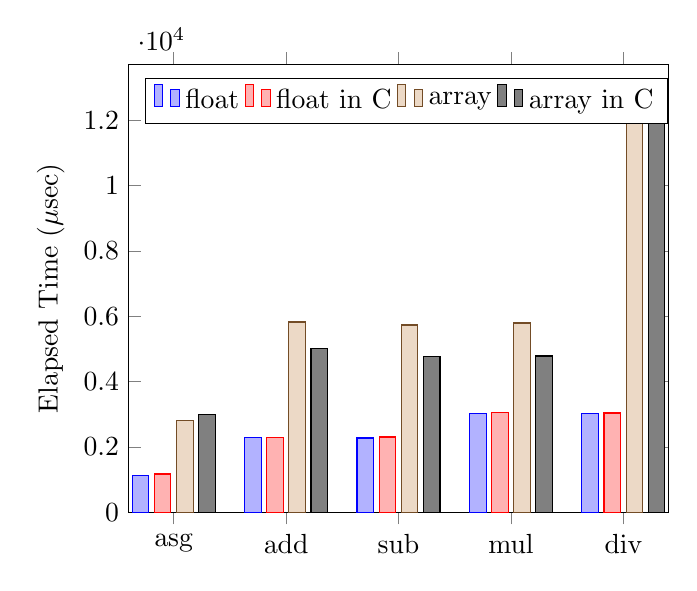
\begin{tikzpicture}
\begin{axis}[
  ybar, bar width=6pt,
  ylabel=Elapsed Time ($\mu$sec),
  symbolic x coords={asg, add, sub, mul, div},
  legend pos=north west, legend columns=4]
\addplot coordinates
  {(asg, 1134.2) (add, 2277.2) (sub, 2271.8) (mul, 3034) (div, 3029.2)};
\addplot coordinates
  {(asg, 1168.6) (add, 2280.8) (sub, 2302.8) (mul, 3044) (div, 3039.2)};
\addplot coordinates
  {(asg, 2800.4) (add, 5823.2) (sub, 5733) (mul, 5792.2) (div, 12575)};
\addplot coordinates
  {(asg, 3000.4) (add, 5008.8) (sub, 4763.2) (mul, 4783.8) (div, 12519.6)};
\legend{float, float in C, array, array in C}
\end{axis}
\end{tikzpicture}

\caption{Comparison of float point arithmetics}
\label{fig:arith}
\end{figure}

\subsubsection{Tuple vs. Record}\label{sec:tuple_record}
{\em Tuple} and {\em Record} are two light-weight data types for encapsulating a
group of data. When translated to intermediate C code, tuple is transformed to
multiple dimensional array and record is transformed to the {\ic struct} type.
Following code illustrates the correspondence in translation of {\ic tuple}
type, {\ic record} type, and their nested constructions.

\begin{lstlisting}
    /* Chapel source */            /* C mapping */
    var tup: (int, int);           int tup[2];
    var nstTup: (tup, tup);        int nstTup[2][2];

    record Rec {var x, y: int;}    struct rec {int x, y;}
    record nstRec {                struct nstRec {
        var x, y: Rec; }               struct rec x, y; }
\end{lstlisting}

As described in \autoref{sec:md_datastruct}, both {\ic tuple} and {\ic
record} can be used to implement vector. \autoref{fig:1d_vector} and
\autoref{fig:2d_vector} show the manipulation performance of 1D and 2D vectors,
respectively. 2D vector is implemented by nested types. The number of vectors is
$10^6$ and we also compare them with a {\em direct C implementation} using array
and {\ic struct}. Results show that using {\ic tuple} has a potential indexing
overhead (up to 50\%) than using {\ic record}, and the increment of overhead by
using nested types is much higher comparing to direct C implementation.

\begin{figure}[t]
\centering
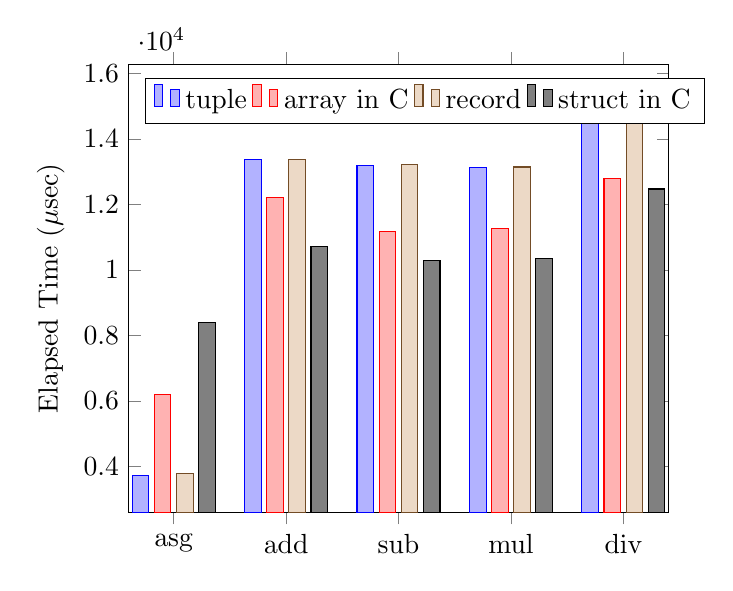
\begin{tikzpicture}
\begin{axis}[
  ybar, bar width=6pt,
  ylabel=Elapsed Time ($\mu$sec),
  symbolic x coords={asg, add, sub, mul, div},
  legend pos=north west, legend columns=4]
\addplot coordinates
  {(asg, 3733.8) (add, 13373.6) (sub, 13202.2) (mul, 13135) (div, 15143.4)};
\addplot coordinates
  {(asg, 6198.2) (add, 12207.6) (sub, 11178) (mul, 11278.8) (div, 12806)};
\addplot coordinates
  {(asg, 3788.4) (add, 13375.2) (sub, 13210.4) (mul, 13145.2) (div, 15115.2)};
\addplot coordinates
  {(asg, 8392.8) (add, 10704.6) (sub, 10299.4) (mul, 10362.4) (div, 12472.4)};
\legend{tuple, array in C, record, struct in C}
\end{axis}
\end{tikzpicture}

\caption{Performance of manipulations on 1D-vectors}
\label{fig:1d_vector}
\end{figure}

\begin{figure}[t]
\centering
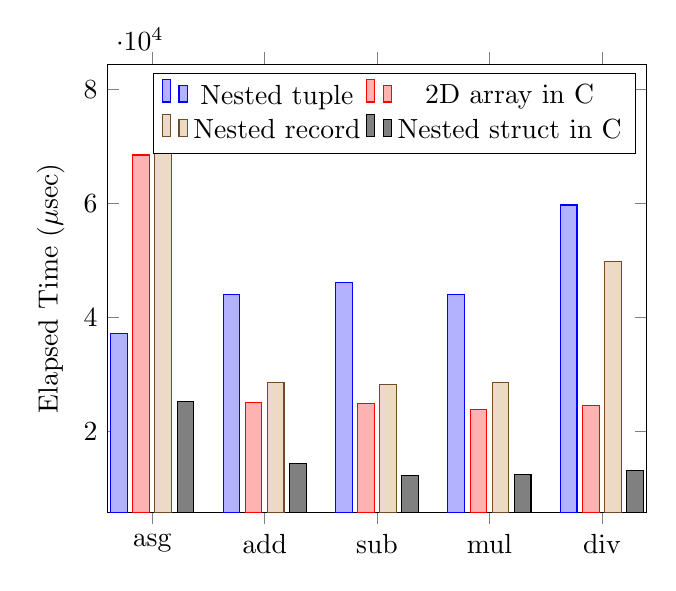
\begin{tikzpicture}
\begin{axis}[
  ybar, bar width=6pt,
  ylabel=Elapsed Time ($\mu$sec),
  symbolic x coords={asg, add, sub, mul, div},
  legend columns=2]
\addplot coordinates
  {(asg, 37227.6) (add, 43990.8) (sub, 46055.6) (mul, 43937.6) (div, 59695)};
\addplot coordinates
  {(asg, 68454.2) (add, 25028.8) (sub, 24933.2) (mul, 23775.2) (div, 24469.8)};
\addplot coordinates
  {(asg, 77836) (add, 28498) (sub, 28265.8) (mul, 28566.2) (div, 49820.6)};
\addplot coordinates
  {(asg, 25209.2) (add, 14292) (sub, 12311.4) (mul, 12413.6) (div, 13181)};
\legend{Nested tuple, 2D array in C, Nested record, Nested struct in C}
\end{axis}
\end{tikzpicture}

\caption{Performance of manipulation on 2D-vectors}
\label{fig:2d_vector}
\end{figure}

\subsection{Domain Indexing}
In Chapel, domain is classified as {\em rectangular domain} and {\em
irregular/associative domain}~\cite{chapelspec}. Rectangular domain describes
multidimensional rectangular index sets, and irregular domain is like
dictionary-style array which can use arbitrary type as index.

To study the performance of domain reference, we compare the throughput of
manipulation on arrays that are defined by rectangular domain and associate
domain. The size of all arrays is set to $10^6$, and the length of a
$n$-dimensional array is $10^{6/n}$. \autoref{fig:array} presents the
experimental results. Generally, using regular domain is much more efficient
(hundreds times faster) than using associate domain because regular domain
typically requires $O(1)$ space~\cite{chapelspec}.
\begin{figure}[t]
\centering
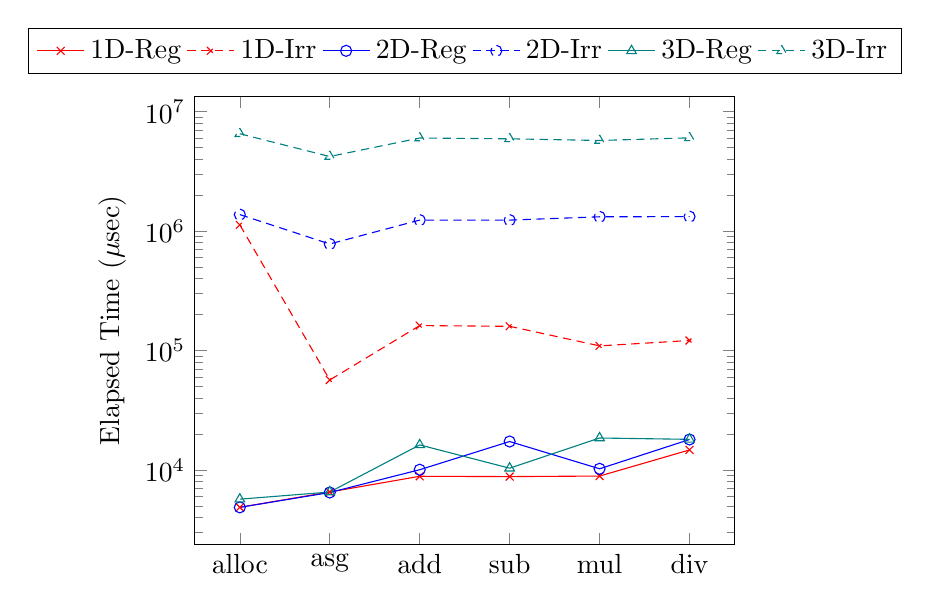
\begin{tikzpicture}
\begin{axis}[
  ymode=log,
  ylabel=Elapsed Time ($\mu$sec),
  symbolic x coords={alloc, asg, add, sub, mul, div},
  legend style={at={(0.5, 1.05)}, anchor=south, legend columns=6}]]
% 1D-Rec
\addplot[mark=x, color=red] coordinates
  {(alloc, 4878.8) (asg, 6555.2) (add, 8872.4) (sub, 8819.2) (mul, 8912.8) 
   (div,14743.4)};
% 1D-Irr
\addplot[mark=x, color=red, style=densely dashed] coordinates
  {(alloc, 1130004.8) (asg, 56809) (add, 162065.2) (sub, 159844) (mul, 109623)
   (div, 121578.4)};
% 2D-Rec
\addplot[mark=o, color=blue] coordinates
  {(alloc, 4873.8) (asg, 6490.8) (add, 10068) (sub, 17344.4) (mul, 10250.8)
   (div, 18036.8)};
% 2D-Irr
\addplot[mark=o, color=blue, style=densely dashed] coordinates
  {(alloc, 1377234.2) (asg, 781581.4) (add, 1238850.4) (sub, 1238424.4)
   (mul, 1319992) (div, 1324668)};
% 3D-Rec
\addplot[mark=triangle, color=teal] coordinates
  {(alloc, 5708.4) (asg, 6549.8) (add, 16246.4) (sub, 10368.6) (mul, 18559)
   (div, 18087.8)};
% 3D-Irr
\addplot[mark=triangle, color=teal, style=densely dashed] coordinates
  {(alloc, 6544416) (asg, 4218638) (add, 6025574) (sub, 5937296) (mul, 5747632)
   (div, 6049830)};
\legend{1D-Reg, 1D-Irr, 2D-Reg, 2D-Irr, 3D-Reg, 3D-Irr}
\end{axis}
\end{tikzpicture}

\caption{Indexing performance of arrays with different domains}
\label{fig:array}
\end{figure}

\subsection{Nested For Loop}\label{sec:nested_loop}
The nested loop is common in scientific calculation, and it can be constructed
using a {\em nested iteration} or {\em zipper iteration} in Chapel. But when the
inner loop depends on the outer loop, the iteration can only use the nested way
because the {\em range literal} is evaluated at once before iterations (see
example below).
\begin{lstlisting}
    // Nested iteration
    for i in [1..I] do  // Inner loop depends on outer loop
      for j in [1..I-1] { .. } 

    // Zipper iteration
    for (i, j) in [1..I, 1..J] do { ... }    // OK
    for (i, j) in [1..I, 1..I-1] do { ... }  // NG
\end{lstlisting}

\autoref{fig:loop} shows the elapsed time of conducing $10^6$ times of
accumulation by using different {\ic for}/{\ic while} constructions. Here,
``{\ic for-for}'' stands for a nested iteration and ``{\ic for2}'' stands for a
zipper iteration. For a $n$-level nested loops, each level is iterated for
$10^{6/n}$ times.
\begin{figure*}[t]
\centering
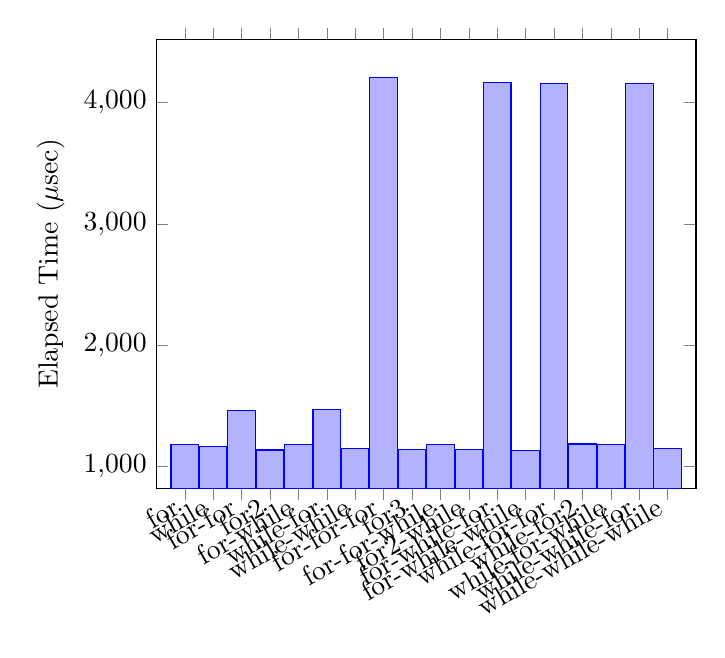
\begin{tikzpicture}
\begin{axis}[ybar,
  x tick label style={rotate=30, anchor=east},
  ylabel=Elapsed Time ($\mu$sec),
  xmin=0, xmax=19,
  xtick={1,2,3,4,5,6,7,8,9,10,11,12,13,14,15,16,17,18},
  xticklabels={for, while, for-for, for2, for-while, while-for,
  while-while, for-for-for, for3, for-for-while, for2-while,
  for-while-for, for-while-while, while-for-for, while-for2, while-for-while,
  while-while-for, while-while-while}]
\addplot coordinates
{(1, 1183) (2, 1166.2) (3, 1464)  (4, 1135.4) (5, 1183) 
 (6, 1467.8) (7, 1145.2) (8, 4209.6) 
 (9, 1136.4) (10, 1182) (11, 1136)
 (12, 4165.6) (13, 1129.4) (14, 4156)
 (15, 1184.8) (16, 1179.4) (17, 4155)
 (18, 1144.6)};
\end{axis}
\end{tikzpicture}

\caption{Performance comparison of traversing various nested loops}
\label{fig:loop}
\end{figure*}

It is clear that the overhead is non-trivial when {\ic for} exists in inner
loops. Following intermediate C code shows that a {\ic for} loop in Chapel is
translated into a {\ic while} loop surrounded by a pair of domain constructor
and destructor procedures which are also iterated by outer loops.

\begin{lstlisting}
    // Transformed C code of the for loop
    chpl__buildDomainExpr2(&loop_domain, ...);
    while (loop_domain) { ... }
    chpl__autoDestroy2(loop_variable, ...);
\end{lstlisting}

Thus, there are three ways to overcome this problem by preventing compiler from
inserting the domain construction procedures.
\begin{itemize}
  \item Define an {\em iterator} by using {\ic iter} function~\cite{chapelspec},
  which preserves the semantics of data parallelism in the {\ic forall}
  loop\footnote{However, the parallel iterator is not available now. It will be
  supported in the future~\cite{chapelspec}.}. 
  \item Use the {\ic while} statement for inner loop, if the inner loop does not
  need to be executed in parallel.
  \item Use zipper iteration, if inner loop is independent of outer loop.
\end{itemize}

\subsection{Molecular Dynamics Applications}

\subsubsection{Serial Execution Performance}
\autoref{fig:fmm_serial} shows the performance of the serial version of
\ac{FMM}. Similar as evaluation results in previous sections, a Chapel program
generally achieves about 50\% of the performance of an identical C program.
Though not shown here, other simpler \ac{MD} programs with fewer array reference
can achieve about 60-70\% performance of the C implementation.

\begin{figure}[t]
\centering
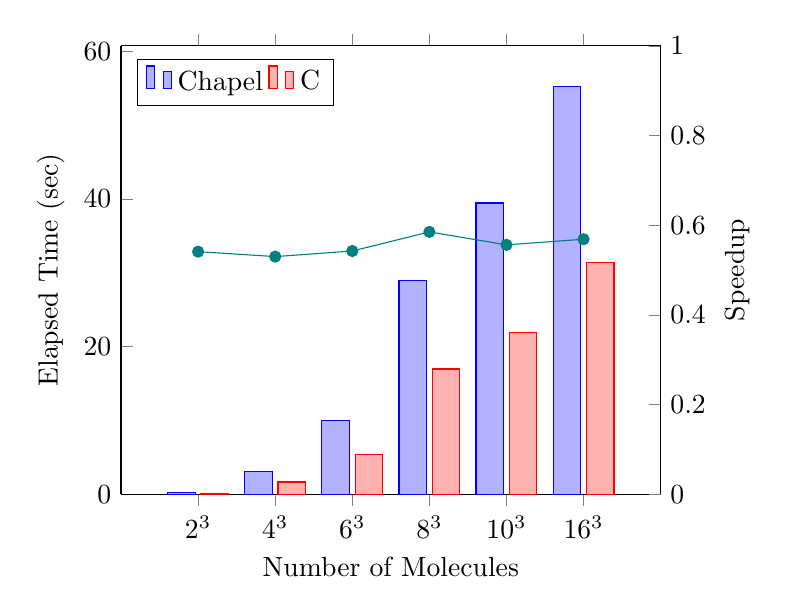
\begin{tikzpicture}
\begin{axis}[ybar, ylabel=Elapsed Time (sec), ymin=0, axis y line*=left,
  xlabel=Number of Molecules,
  xmin=0, xmax=7, xtick={1,2,3,4,5,6},
  xticklabels={$2^3$, $4^3$, $6^3$, $8^3$, $10^3$, $16^3$},
  legend pos=north west, legend columns=2]
\addplot coordinates
{(1, 0.1738) (2, 3.0888) (3, 9.93) (4, 28.9722) (5, 39.4486) (6, 55.2144)};
\addplot coordinates
{(1, 0.094) (2, 1.6366) (3, 5.385) (4, 16.9468) (5, 21.9326) (6, 31.3942)};
\legend{Chapel, C}
\end{axis}

\begin{axis}[xmin=0, xmax=7, ymin=0, ymax=1,
axis y line*=right, axis x line=none, ylabel=Speedup]
\addplot[mark=*, color=teal, update limits=false] coordinates
{(1, 0.54085) (2, 0.52984) (3, 0.54229) (4, 0.58493) (5, 0.55598) (6, 0.56859)};
\end{axis}
\end{tikzpicture}

\caption{Performance of serial \acs{FMM}}
\label{fig:fmm_serial}
\end{figure}

\subsubsection{Parallel Execution Performance}
To parallelize a serial program, parallel statements and synchronization are
inserted. Figure~\ref{fig:fmm_breakdown} shows the performance breakdown of
\ac{FMM} phases by a serial version and a parallelized version (but executed
serially) \ac{FMM} programs. For the most computation intensive part (\ie
{\ic multipoleCalc} phase), the parallelization can introduces 5 times of
overhead because lock is used in a heavy loop part.
\begin{figure}[t]
\centering
% huscs, N=32*32*32, numThreadsPerLocale=1, step=1
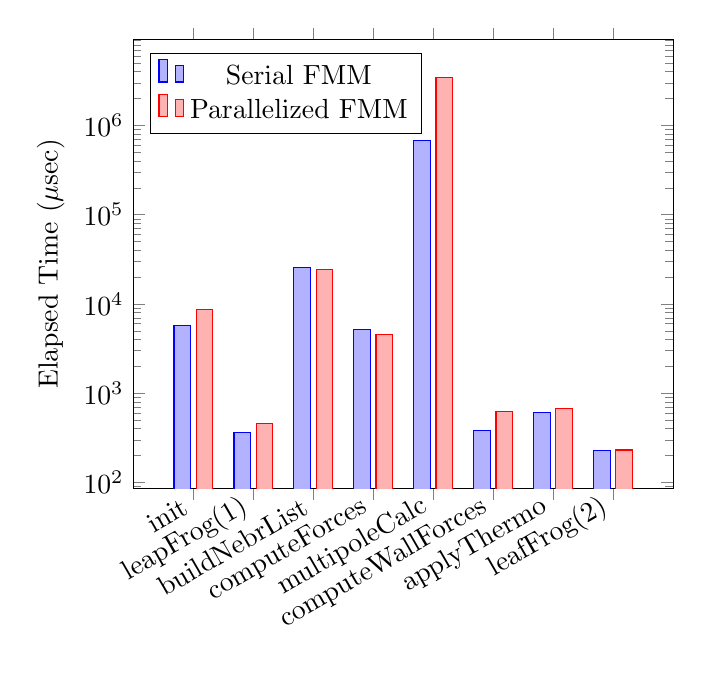
\begin{tikzpicture}
\begin{axis}[
  ymode=log, ybar, bar width=6pt,
  ylabel=Elapsed Time ($\mu$sec),
  xmin=0, xmax=9, xtick={1, 2, 3, 4, 5, 6, 7, 8},
  xticklabels={init, leapFrog(1), buildNebrList, computeForces, multipoleCalc,
    computeWallForces, applyThermo, leafFrog(2)},
  x tick label style={rotate=30, anchor=east},
  legend pos=north west, legend columns=1]
\addplot coordinates
  {(1, 5691) (2, 360) (3, 25388) (4, 5145) (5, 674491) (6, 385) (7, 603) 
   (8, 227)};
\addplot coordinates
  {(1, 8631) (2, 462) (3, 24151) (4, 4550) (5, 3480940) (6, 618) (7, 680) 
   (8, 231)};
\legend{Serial FMM, Parallelized FMM}
\end{axis}
\end{tikzpicture}

\caption{Serial performance breakdown of serial \ac{FMM} and parallelized \ac{FMM}}
\label{fig:fmm_breakdown}
\end{figure}

Figure~\ref{fig:fmm_scale} shows the scalability of parallel \ac{FMM} for
different number of threads and problem sizes.
Figure~\ref{fig:fmm_scale_breakdown} illustrates the scalability of each phase
for $N=32^3$.  For a small problem size (\eg $N=8^3$), the performance drops
down when the number of threads exceed 4 because there are less calculations for
long range interactions and the computation for short range is dominant. When
there are more molecules, which suggests larger space, the performance scales up
to 8 threads. However, the speedup only achieves 4 for 8 threads, this is
because an lock existing in {\ic multipoleCalc} phase leads to significant
overhead. We are currently developing a new algorithm for this phase to remove
the usage of lock.

\begin{figure}[t]
\centering
% huscs, steps=10
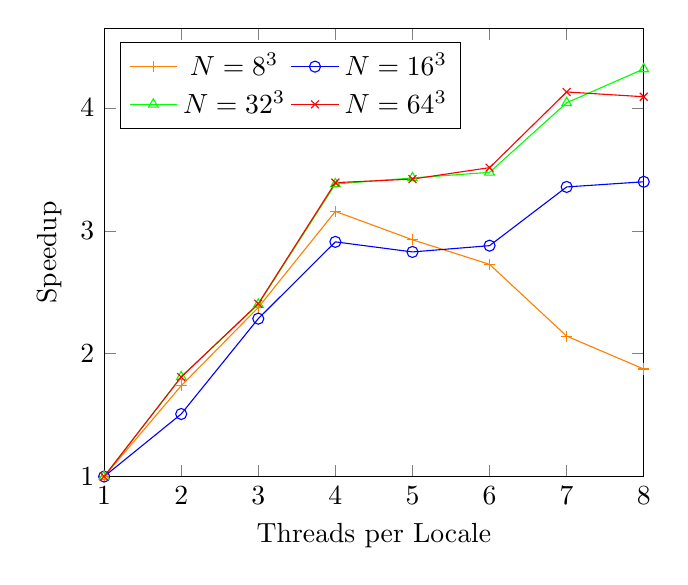
\begin{tikzpicture}
\begin{axis}[
  ylabel=Speedup, ymin=1,
  xmin=1, xmax=8, xtick={1, 2, 3, 4, 5, 6, 7, 8},
  xlabel=Threads per Locale,
  legend pos=north west, legend columns=2]
% N=8**3
\addplot[mark=+, color=orange] coordinates
  % 0.24  0.138 0.101 0.076 0.082 0.088 0.112 0.128
  {(1, 1) (2, 1.739) (3, 2.376) (4, 3.158) (5, 2.927) (6, 2.727) 
   (7, 2.143) (8, 1.875)};
% N=16**3
\addplot[mark=o, color=blue] coordinates
  % 0.809 0.536 0.354 0.278 0.286 0.281 0.241 0.2380
  {(1, 1) (2, 1.509) (3, 2.285) (4, 2.910) (5, 2.828) (6, 2.879) 
   (7, 3.357) (8, 3.399)};
% N=32**3
\addplot[mark=triangle, color=green] coordinates
  % 34.859, 19.244, 14.521, 10.310, 10.163, 10.028, 8.625, 8.075
  {(1, 1) (2, 1.811) (3, 2.401) (4, 3.381) (5, 3.430) (6, 3.476) 
   (7, 4.042) (8, 4.317)};
% N=64**3, STEP=2
\addplot[mark=x, color=red] coordinates
  % 440.885 243.609 183.189 129.985 128.869 125.48  106.816 107.761
  {(1, 1) (2, 1.810) (3, 2.407) (4, 3.392) (5, 3.421) (6, 3.514) 
   (7, 4.13) (8, 4.091)};
\legend{$N=8^3$, $N=16^3$, $N=32^3$, $N=64^3$}
\end{axis}
\end{tikzpicture}

\caption{Scalability of parallelized \ac{FMM}}
\label{fig:fmm_scale}
\end{figure}

\begin{figure}[t]
\centering
% huscs, N=32*32*32, numThreadsPerLocale=1,2,3,..,8, step=1
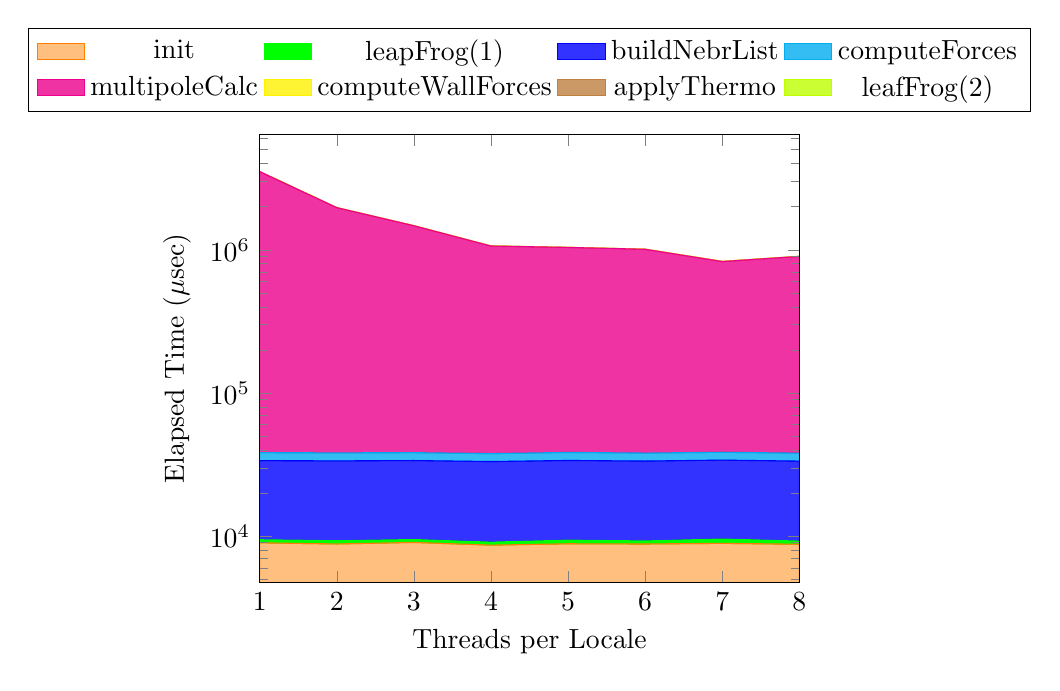
\begin{tikzpicture}
\begin{axis}[
  stack plots=y, area style, enlarge x limits=false,
  ymode=log,
  ylabel=Elapsed Time ($\mu$sec),
  xmin=1, xmax=8, xtick={1, 2, 3, 4, 5, 6, 7, 8},
  xlabel=Threads per Locale,
  legend style={at={(0.5, 1.05)}, anchor=south, legend columns=4}]
\addplot[orange, fill=orange, fill opacity=0.5] coordinates % init
  {(1, 8989) (2, 8825) (3, 9045) (4, 8658) (5, 8850) (6, 8821) (7, 8914) 
   (8, 8783)} \closedcycle;
\addplot[green, fill=green] coordinates % leapFrog(1)
  {(1, 454) (2, 468) (3, 426) (4, 425) (5, 530) (6, 440) (7, 637) (8, 457)}
  \closedcycle;
\addplot[blue, fill=blue, fill opacity=0.8] coordinates % buildNebrList
  {(1, 24268) (2, 24276) (3, 24282) (4, 24134) (5, 24417) (6, 24213) (7, 24434) 
   (8, 24207)} \closedcycle;
\addplot[cyan, fill=cyan, fill opacity=0.8] coordinates % computeForce
  {(1, 4612) (2, 4618) (3, 4564) (4, 4528) (5, 4653) (6, 4581) (7, 4567) 
   (8, 4549)} \closedcycle;
\addplot[magenta, fill=magenta, fill opacity=0.8] coordinates % multipoleCalc
  {(1, 3480480) (2, 1932990) (3, 1434660) (4, 1025450) (5, 1000760) 
   (6, 970789) (7, 789904) (8, 861565)} \closedcycle;
\addplot[yellow, fill=yellow, fill opacity=0.8] coordinates % computeWallForce
  {(1, 727) (2, 840) (3, 738) (4, 659) (5, 509) (6, 619) (7, 811) (8, 450)}
  \closedcycle;
\addplot[brown, fill=brown, fill opacity=0.8] coordinates % applyThermo
  {(1, 647) (2, 724) (3, 798) (4, 690) (5, 670) (6, 679) (7, 906) (8, 649)}
  \closedcycle;
\addplot[lime, fill=lime, fill opacity=0.8] coordinates % leapFrog(2)
  {(1, 233) (2, 380) (3, 399) (4, 340) (5, 335) (6, 364) (7, 447) (8, 334)}
  \closedcycle;
\legend{init, leapFrog(1), buildNebrList, computeForces, multipoleCalc,
    computeWallForces, applyThermo, leafFrog(2)},
\end{axis}
\end{tikzpicture}

\caption{Parallel performance breakdown of parallelized \ac{FMM}}
\label{fig:fmm_scale_breakdown}
\end{figure}

\subsection{Source Lines of Code}
Figure~\ref{fig:loc} shows the head-to-head comparison of \ac{LOC} between
serial programs of our Chapel and original C implementation. Using Chapel saves
20-40\% effort to develop a program. Note that the parallel version of programs
in Chapel only introduce a small fraction of additional code. For example, our
parallelized \ac{FMM} program has only 3\% more lines of code than the serial
version, which demonstrates that expressive of describing parallelism by Chapel.

\begin{figure}[t]
\centering
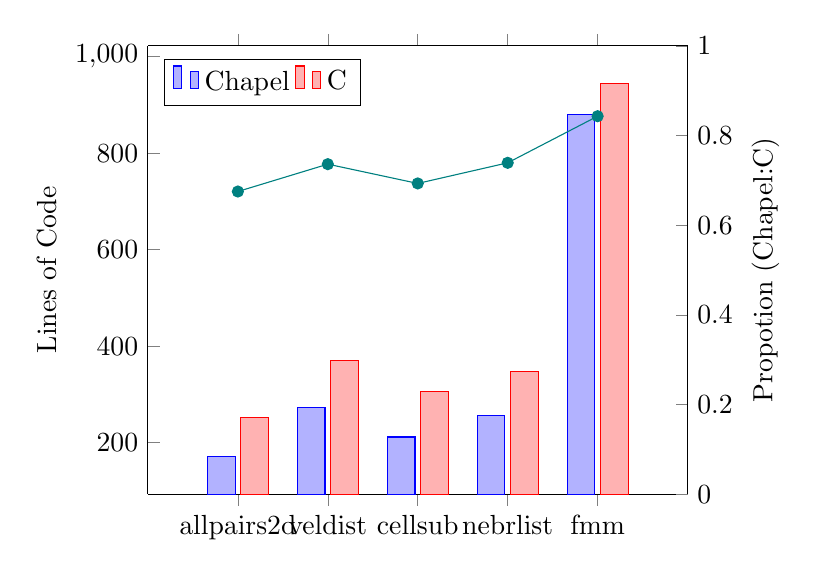
\begin{tikzpicture}
\begin{axis}[ybar, axis y line*=left,
  ylabel=Lines of Code, legend pos=north west, legend columns=2, xmin=0, xmax=6,
  xtick={1,2,3,4,5}, 
  xticklabels={allpairs2d, veldist, cellsub, nebrlist, fmm}]
\addplot plot coordinates
{(1, 171) (2, 273) (3, 212) (4, 257) (5, 880)};
\addplot plot coordinates
{(1, 253) (2, 371) (3, 306) (4, 348) (5, 945)};
\legend{Chapel, C}
\end{axis}

\begin{axis}[axis y line*=right,
  axis x line=none,
  ylabel=Propotion (Chapel:C),
  xmin=0, xmax=6, ymin=0, ymax=1]
\addplot[mark=*, color=teal] plot coordinates
{(1, 0.675) (2, 0.736) (3, 0.693) (4, 0.739) (5, 0.843)};
\end{axis}
\end{tikzpicture}

\caption{Comparison of lines of code of serial MD programs}
\label{fig:loc}
\end{figure}
